\chapter{Distributed Computing}

\section{Introduction}

A distributed system is composed of many autonomous interconnected entities with their own hardware (memory, CPU). The entities can send messages to each other via the network.

The natural way to represent a DS is a graph. There are many models to describe different aspects of the system. They have to deal with the following issues:

\begin{enumerate}
\item Communication. Usually communication is very expensive, its cost dominates all other costs. Hence it is typically assumed that communication is the only cost that occurs.
\item Fault Tolerance. In large computer networks it's common that a few nodes fail during the computation. Robustness against this is desirable. Results should be reasonable even if single entities fail.
\item Locality. Networks change over time, communicating these changes to all nodes would be too costly. It's better to design algorithms that only rely on local information.
\item Synchronization. Individual entities can have different hardware and solve problems at different speeds. It's good if algorithms don't have to assume synchronous computation.
\item Symmetry breaking. Nodes have to be made distinguishable.
\end{enumerate}

\section{Vertex Coloring}

Given an undirected graph $G=(V,E)$ we want to find a colouring, i.e. an assignment of colours $c_v$ to the vertices $v\in V$, such that no two adjacent vertices have the same colour.

This is useful for symmetry breaking. For example cellphones that communicate with the same cell have to choose different frequencies.

We will assume that initially all nodes are equipped with a unique ID from $[1,n]$. Typically each ID uses $O(\log n)$ bits. Obviously the IDs are a valid colouring. We want to try to use fewer colours, if possible the minimal number.

\begin{Def}[Chromatic Number] The chromatic number $\chi(G)$ of a graph is the minimal number of colours needed in any valid colouring of G.
\end{Def}

Computing the chromatic number is NP-complete\footnote{It's actually one of \href{http://www.cs.berkeley.edu/~luca/cs172/karp.pdf}{Karp's original 21 complete problems}}. Hence we want to try to find some approximate solution.

A simple, sequential algorithm assigns colours greedily:

\begin{lstlisting}
Greedy(graph G)
while $\exists$ uncoloured vertex v
	colour v with min ([1,n] - colours(neighb(v)))
\end{lstlisting}

\begin{thm} The greedy algorithm stops after $n$ steps and produces a valid colouring and uses at most $\Delta(G)+1$ colours\footnote{$\Delta(G)$ is the maximal degree of the graph}.
\end{thm}

\begin{pr} It is clear that the algorithm stops in $n$ steps, since in each iteration the number of vertices decreases by one. 

Correctness is given by an inductive argument. During the execution the coloured subgraph has a valid colouring, since we assign colours that don't occur in the neighbourhood.

Finally $\Delta(G)+1$ is an upper bound for the number of colours since there is always a free colour in the set $[1,\Delta(G)+1]$.
\end{pr}

We want to construct a distributed algorithm that uses the same ideas to reduce the number of colours. In a distributed setting, each node runs the following code independently:

\begin{lstlisting}
First-Free(coloured neighbourhood, vertex v)
	give v the smallest available colour
\end{lstlisting}

This algorithm can fail if two adjacent vertices choose the colour at the same time under certain circumstances, as depicted in figure \ref{fig:first-free-error}.

\begin{figure}
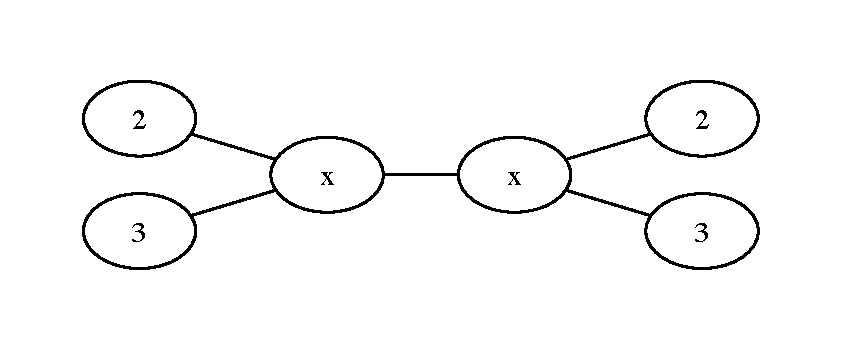
\includegraphics[width=0.5\linewidth]{./images/graph1}
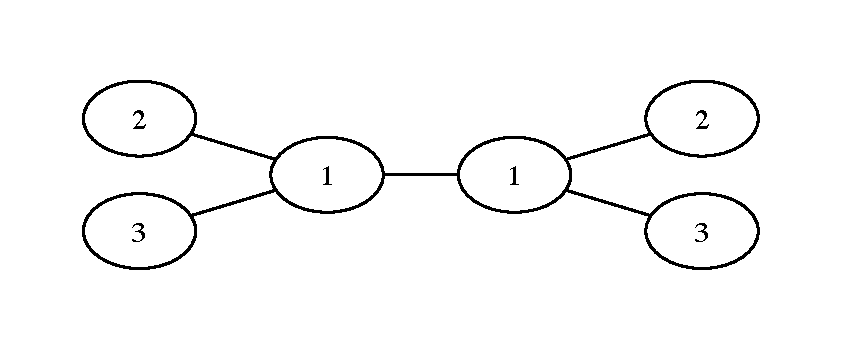
\includegraphics[width=0.5\linewidth]{./images/graph11}
\caption{If the nodes labelled with x have high IDs and choose simultaneously they produce an invalid colouring.}
%n1 2
%n2 x
%n3 3
%n4 10
%n5 2
%n6 3
%n1 -- n2
%n2 -- n3
%n2 -- n4
%n4 -- n5
%n4 -- n6
%
%n1 and n2 choose colours simultaneously, both get 1.
\label{fig:first-free-error}
\end{figure}

It depends on the model how we can deal with this. Either we have the means for synchronisation, or we don't.

\begin{Def}[Synchronous Distributed Algorithm] During one unit of time an entity in a SDA can execute (in any order) the following things
\begin{itemize}
\item Perform local computations
\item Send messages
\item Receive messages
\end{itemize}

As long as each is of "reasonable" complexity.
\end{Def}

We can express the algorithm as a SDA like this:

\begin{lstlisting}
Reduce
	send own ID to all neighbours
	receive IDs from all neighbours
	while $\exists$ uncoloured neighbour with larger ID
		send "uncoloured" to all neighbours
		receive messages from neighbours
	colour thyself with First-Free
	send the colour to neighbours
\end{lstlisting}

\begin{thm} Reduce is correct, i.e. it produces a valid colouring after at most $n$ rounds. The number of colours used is upper bounded by $\Delta(G)+1$. 
\end{thm}

\begin{pr} In every round there is a vertex that has the highest ID and thus gets coloured. Hence at most $n$ rounds are used. Since we use First-Free to assign the colours, the number of colours is $\leq \Delta+1$.

This algorithm always produces a correct colouring, since no two vertices that are connected by an edge choose their colour simultaneously. One of them will always have a higher ID and prevent the other one from choosing.
\end{pr}
